\documentclass[12pt]{report}
\usepackage{xcolor}
\usepackage{fullpage}
\usepackage{graphicx}
\usepackage{fixltx2e}
\usepackage[margin=0.5in]{geometry}
\begin{document}
	\definecolor{mycolor1}{RGB}{210,210,255}
\centering{\colorbox{mycolor1}{\textbf{\Huge{\hspace{10pt}KARTIK VASHISHT}}}

\colorbox{mycolor1}{\textbf{\Large{Electronics and Communication Engineering}}}

\vspace{7pt}
\textbf{\large{Address(Permanent): E-44 Kilokeri opp. Maharani Bagh, New Delhi-14 }}

\textbf{\large{Address(Corresponding): B-258, Hostel No.10 (Visvesvara Bhawan),\qquad}} 
			
\textbf{\large{\hspace{170pt} National Institute of Technology, Kurukshetra}}

\vspace{10pt}
\colorbox{white}{\textbf{\large{Email: karvash.kv@gmail.com \qquad \qquad Contact No.: 8295156523/9729045096}}}

\vspace{10pt}
\begin{figure}
	\centering
	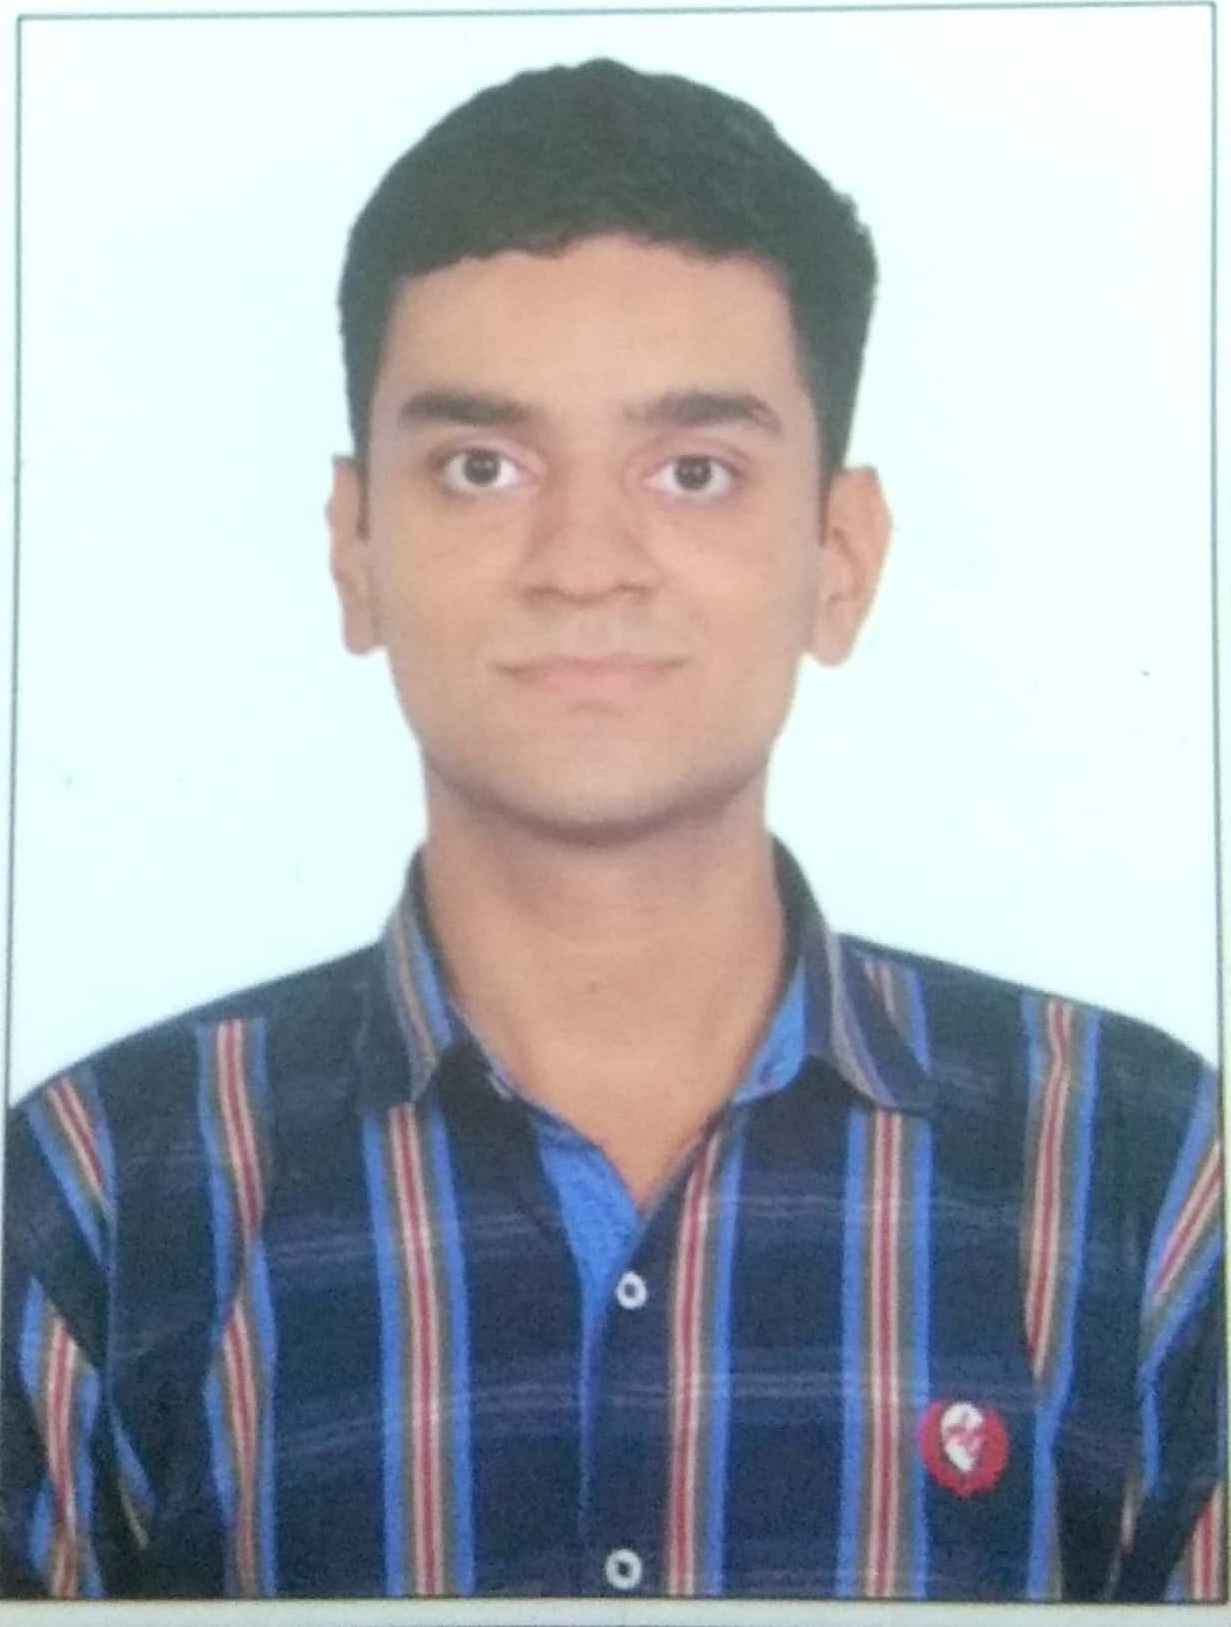
\includegraphics[scale=0.13]{Self.jpg}
\end{figure}

\vspace{20pt}
\textbf{\large{\underline{Career Objectives:}}}
\large{ The future objective and aims of my life are to gain as much knowledge as I can and use that knowledge in implementing solutions and engineering things that can help in solve in daily life problems. I am enthusiastic about electronics and communication and want to explore deep in this field. I want to contribute toward making the world a simpler, better, safer place. So I want to learn and work with new skills, fields, gadgets and experts in my future. }

\vspace{15pt}
\textbf{\large{\underline{Education:}}}

\vspace{6pt}
\begin{tabular}{||c|c|c|c|c|c|c|c||}
	\hline
	\textbf {Exam} & \textbf {Institution} & \textbf {Year of Passing} & \multicolumn{5}{ c|| }{\textbf {GPA or \%}} \\
	\hline
	B.Tech. & NIT, Kurukshetra & 2020 & \small 5\textsuperscript{th} S & \small 4\textsuperscript{th} S & \small 3\textsuperscript{rd} S & \small 2\textsuperscript{nd} S & \small 1\textsuperscript{st} S  \\ \cline{4-8}
	& & (still not & 9.0 & 9.592 & 9.4 & 9.48 & 9.14 \\ \cline{4-8}
	& & completed) & \multicolumn{5}{ c|| }{Aggregate CGPA: 9.38} \\
	\hline
	12\textsuperscript{th} Board & Navodaya Bal Sr. Sec. & 2016 & \multicolumn{5}{ c|| }{89.8\%} \\ (RBSE) & School, Kota, Rajasthan & &\multicolumn{5}{ c|| }{}\\
	\hline
	10\textsuperscript{th} Board & Cambridge School, & 2014 & \multicolumn{5}{c||}{10}\\(CBSE) & Srinivaspuri, New Delhi & &\multicolumn{5}{c||}{}\\
	\hline
\end{tabular}

\vspace{3pt}
\normalsize{. \hspace{450pt} *S - Semester}

\vspace{80pt}
\textbf{\large{\underline{Projects:}}}
\begin{enumerate}
	\large{\item Made a prototype on Smart Irrigation System based on soil moisture and temperature that can be controlled automatically and manually from a remote location.}
	\item 	Created a TIC-TAC-TOE with the help of Basic Image Processing using Python.
	\item Gesture Controlled Robot using Accelerometer and Bluetooth Sensor, controlled using remote or Self Made Mobile App (using MIT app inventor).
	\item	Obstacle Detection and Avoidance Robot using ultrasonic sensor. 
	\item Created Smart lighting, Christmas lighting, Emergency alarms and many models using Arduino.
	\item Created a Best-out-of-Waste Hydraulics bridge using syringe and ice cream sticks.
	\item Created an Electricity Generator using Dynamo and rotating wheel.
	\item Designed Line-Following Robot with and without microcontroller.
	
\end{enumerate}


\end{document}